\subsection{Intrusion Detection Systems / Intrusion Prevention Systems}
Datensicherheit beschreibt eine Herangehensweise, das in erster Linie das Ziel verfolgt, ein System gegen vielzählige Verstöße zu schützen. Dies ist in den meisten Fällen nur schwer möglich, da die Systeme sehr komplex sein können. So gut wie jedes System weißt Sicherheitsschwachstellen auf, welche zu schlimmen Problemen führen können.
Als Antwort auf diese Sicherheitsprobleme, welche die Funktionsweise des Systems beinträchtigen können, etablierte sich eine neue Vorangehensweise. Die sogenanten Intrusion Detection Systems.
IDS überwachen Systeme auf eventuelle Sicherheitsverstöße und automatisieren die Analyseprozesse von Ereignissen. Somit können plötzliche Sicherheitsprobleme aufgedeckt werden.\cite{haystack_ids}
Ein IDS besitzt 3 folgenden logische Komponenten: \cite{IDS_Book_2}

\begin{itemize}
    \item \textbf{Sensoren}: Die Sensoren sind für das Sammeln der Daten zuständig. Der Input für den Sensor kann jedes mögliche Teil eines Systems sein, das Beweise für eine Intrusion enthält.\cite{IDS_Book_2}\bigbreak
    \item \textbf{Analysatoren}: Empfangen den Input von Sensoren oder anderen Analysatoren. Sie haben die Aufgabe, zu bestimmen ob eine Intrusion eingetreten ist. Der Output der Analysatoren ist eine Indikation, dass eine Intrusion stattgefunden hat.\cite{IDS_Book_2}\bigbreak
    \item \textbf{Benutzerschnittstelle}: Stellt den Benutzer die Möglichkeit dar, den Output der Analysatoren betrachten zu können oder das Verhalten des System zu modifizieren.\cite{IDS_Book_2}\bigbreak
\end{itemize}

Grundsätzlich können Intrusion Detection Systems in 2 Hauptkategorien eingeteilt werden. Host-based und Network-based IDS.\cite{IDS_Book_1}
In diesem Abschnitt wird generell erklärt, was Host-basierte und Netzwerk-basierte Intrusion Detection Systems sind, mit einigen Beispiele.

\subsection{Host-based Intrusion Detection Systems}
HIDS (Host basierten IDS) setzen den Fokus auf die Aktivitäten eines einzigen Hosts. Sie fügen verletzlichen oder sensitiven Systemen, wie Datenbank-Servern oder administrativen Systemen, eine spezielle Sicherheits-Ebene hinzu. Das HIDS überwacht, auf versch. Art und Weise, Aktivitäten auf dem System. In einigen Fällen kann somit ein Angriff aufehalten werden, bevor er überhaupt Schaden verursacht. \cite{IDS_Book_1} \cite{IDS_Book_2}
Die Hauptaufgabe eines HIDS ist es, mit Regeln und Richtlinien, Protokolldateien zu durchsuchen und diese zu markieren, falls potentiell bösartige Verhaltensmuster erkennt werden.
\clearpage
HIDS können eine weitreichende Menge an Bedrohungen identifizieren \cite{hids_url_2}. Dazu gehören :

\begin{itemize}
  \item Unautorisiertes Einloggen und Zugriffsversuche\bigbreak
  \item Installation von unerwünschten Anwendungen\bigbreak
  \item Privileg-Eskalation\bigbreak
  \item Rogue-Processes\bigbreak
  \item Modifizieren der Binärdaten, Daten und Konfigurationsdateien von Anwendungen\bigbreak
  \item Kritische Dienste die gestoppt wurden oder nicht gestartet werde konnten\bigbreak
\end{itemize}
Der primäre Vorteil von HIDS ist diese interne und externe Bedrohungen identifizieren können, was nicht mit NIDS oder Firewalls möglich wäre.
Ein fundamentaler Bestandteil der Intrusion Detection ist der Sensor, der bestimmte Daten sammelt und diese zum Analysieren an das IDS weiterleitet. Das Thema Sensoren wird in einem späteren Abschnitt genauer erläutert.
Die meisten HIDS nutzen einen Kombination aus Signatur/Heuristik basierten und Anomalie basierten IDS.\cite{hids_url_1}
\textbf{Signatur/Heuristik basierte IDS} suchen nach ihnen schon bekannten Mustern, Identitäten oder spezifische Intrusion-Events, welche über eine Datenbank erkannt werden.\cite{hids_url_1}
\textbf{Anomalie basierte IDS} sind im Gegensatz zu den Signatur basierten IDS mehr auf die Analyse von vertrauenswürdigen Verhalten basiert. Hierzu wird Machine Learning genutzt um bösartiges Verhalten zu markieren.\cite{hids_url_1}

\subsection{Network-based IDS}
Sie analysieren den Verkehr an bestimmten stellen eines Netzwerkes. Der Datenverkehr im Netzwerk wird Paket für Paket,in Echtzeit, oder nahe an Echtzeit, überprüft. 
Durch das einsetzen von sogenannten Netzwerkkarten kann ein N-IDS den Datenverkehr überwachen und somit alle Hosts schützen, die mit diesem Netzwerk verbunden sind.
Das Ziel von NIDS ist es Intrusionsmuster zu indentifizieren.
Im Kontrast zu Host-based IDS sieht man, dass nicht die Aktivitäten eines Nutzers oder einer Software überprüft werden, sondern der Datenverkehr zu einem verletzbaren Netzwerk.
\cite{IDS_Book_1} \cite{IDS_Book_2}
\bigbreak
Mit der erhöhten Nutzung von Verschlüsselungsmethoden fällt es NIDS schwerer, auf bestimmte Inhalte zugreifen zu können, was teilweise ihre Funktionalität einschränken kann. Während sie also eine wichtige Rolle in der Sicherheit eines Netzwerkes spielen, sind sie nur ein Teil der gesamten Lösung \cite{IDS_Book_2}. Eine herkömmliche NIDS-Einrichtung besteht aus einer Menge von Sensoren um den Datenverkehr zu überwachen, einem oder mehreren Server/n für das Verwalten der NIDS-Funktionen und einer oder mehrerer Verwaltungskonsolen für die Benutzerschnittstelle. \cite{IDS_Book_2}
Ein Beispiel für ein NIDS ist Snort. 
\textbf{Snort} ist ein vollständig ausgestattetes open-source Intrusion Prevention System\cite{snort_url}. Kurzgesagt handelt es sich bei Snort um einen "Packet Sniffer" (dt. Paketschnüffler) oder "Packetlogger". 
1998 schrieb Marty Roesch ein Packet Sniffer names APE, zu der Zeit nur für Linuxsysteme. Trotz der tollen Funktionalitäten wollte Roesch einen Sniffer erschaffen, der zudem folgende zusätzliche Eigenschaften haben sollte:\cite{snort_book_1}

\begin{itemize}
  \item funktioniert auf mehreren Betriebssystemen\bigbreak
  \item nutzt einen sog. hexdump payload dump\bigbreak
  \item zeigt alle untersch. Netzwerkpakete auf die selbe Weise an\bigbreak
\end{itemize}
Zu diesem Zeitpunkt wurde Snort nur für Packet-Sniffing genutzt. Roesch nutzt das Tool um seine Modem-Verbindung zu überwachen und seine eigenen Netzwerkanwendung zu debuggen. 1999 wurde Snort dann um eine Signatur-basierte Analyse (oder Regelbasierte-Analyse) Funktionalität erweitert. Ab hier konnte es dann schon als leichtgewichtiges IDS eingesetzt werden.\cite{snort_book_1}

\subsection{Verteilte/Hybrid Intrusion Detection Systems}
In den vergangenen Jahren entwickelte sich das Konzept der Interkommunikation zwischen IDS immer weiter. Es entstanden Schemas, in denen verteilte Systeme miteinander kooperieren, um gemeinsam Intrusionen identifizieren zu können und sich an verändernde Angriffe anpassen zu können. Hierbei werden die Informationsquellen aus den HIDS mit denen aus NIDS kombiniert, um die Intrusionserkennung zu verwalten und koordinieren.
\bigbreak
Ein Beispiel eines solchen hyriden Systems ist das von Intel entwickelte Schema, bekannt als Autonomic Enterprise Security.
\begin{figure}[h]
\center
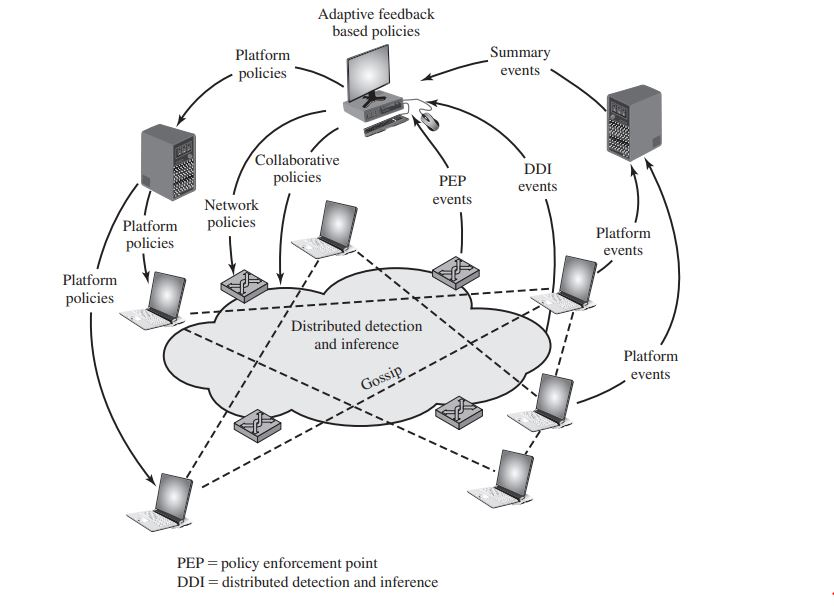
\includegraphics[width=1\textwidth]{img/hybrid_IDS.JPG}
\caption{Beispiel einer Autonomic Enterprise Security \cite{IDS_Book_2}} \label{fig2}
\end{figure}
Fig. 1 stellt den Vorgang dar. Hier werden nicht nur Perimeter-Abwehrmechanismen wie Firewalls oder Host-basierted Verteidiungen eingesetzt. Stattdessen wird jeder Host und jedes Netzwerkgerät (e.g. Router) als eigener sensor betrachtet und besitzt eine eigenen Sensor-Software. Die Sensoren in diesem verteilten System können untereinandern Informationen austauschen um den aktuellen Zustand des Netzwerks zu bestimmen.\cite{IDS_Book_2}
Intel Designer haben die folgenden Motivation zu diesem Vorgang offengelegt:

\begin{enumerate}
    \item Einzelne bereitgestellte IDS können Netzwerk-basierte Angriffe verpassen oder sind zu langsam um die potientielle Attacke zu erkennen. Der Einsatz von mehreren gleichzeitigen IDS ergab eine größere Abdeckung und eine schneller Reaktion auf Angriffe.\bigbreak
    \item Die Analyse des Datenverkehrs auf Host-level stellt eine Umgebung zur Verfügung, in der es weniger Datenverkehr gibt, als auf Netzwerkgeräten wie z.B. Routern. Somit stehen Angriffsmuster besser hervor.\bigbreak
    \item Host-basierte Detektoren können umfangreicheren Datensätze zum Vorteil nutzen. \bigbreak
\end{enumerate}
\subsection{Sensoren}

Wie vorhin schon erwähnt sammelt ein Sensor im Kontext der IDS Daten aus einer Datenquelle. Übliche Datenquellen sind: \cite{IDS_Book_2}

\begin{itemize}
    \item \textbf{System call traces}: Beinhalten Sequenzen von Systemaufrufen von Prozessen. \cite{IDS_Book_2}\bigbreak
    \item \textbf{Log-Dateien}: Die meisten Betriebssysteme besitzen Software die Informationen über Nutzeraktivitäten sammelt.\cite{IDS_Book_2}\bigbreak
    \item \textbf{Prüfsumme der Datenintegrität}: Eine Möglichkeit, Nutzeraktivität auf einem System zu identifizieren, ist es regelmäßig kritische Dateien auf Änderungen zu analysieren. Hierbei wird die aktuelle kryptographische Prüfsumme der Dateien mit schon zuvor bekannten, korrekten Prüfsummen verglichen.\cite{IDS_Book_2}\bigbreak
    \item \textbf{Registry Zugang}: Eine Methode die auf Windows-Systemen genutzt wird. Hierbei wird der Zugang auf die Registry überwacht.\cite{IDS_Book_2}\bigbreak
\end{itemize}
Nachdem die Daten gesammelt wurden, werden zuerst ungewollte Informationen ausgefiltert. Dannach werden die übrigen Informationen in einem standardisierten Format bereitgestellt und diese zuletzt an das IDS zur Analyse weitergereicht.\cite{IDS_Book_2}
Sensoren können in 2 verschiedenen Modi eingesetzt werden. Inline und passiv.\cite{IDS_Book_2}

\subsubsection{Inline Sensoren:}
Ein Inline-Sensor wird in das Netzwerksegment eingeführt um den Verkehr zu überwachen. Jeglicher Verkehr muss diesen Sensor passieren. Mit Inline-Sensnoren können Attacken blockiert werden sobald sie aufgespürt wurden. In so einem Fall führt das System gleichzeitig eine Intrusion Detection und eine Intrusion Prevention durch\cite{url_sensors}\cite{IDS_Book_2}

\subsubsection{Passive Sensoren:}
Normalerweise werden im Allgemeinen meist passive Sensoren genutzt. Im Gegensatz zu Inline-Sensoren überwachen diese nicht direkt den Netzwerk-Verkehr, sondern nur eine Kopie davon. Der eigentliche Verkehr passiert diesen Sensor nicht. Diese Vorgehen ist insgesamt effizienter als das von Inline-Sensoren, da hier kein zusätzlicher Bearbeitungsschritt hinzugefügt wird, der zur Paketverzögerung beiträgt.\cite{url_sensors}\cite{IDS_Book_2}
\begin{figure}
\center
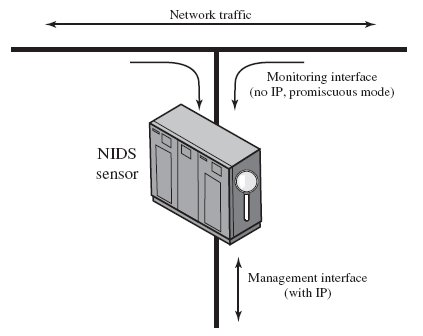
\includegraphics[width=0.5\textwidth]{img/passive_sensor.jpg}
\caption{Illustration eines passiven NIDS Sensors \cite{IDS_Book_2}} \label{fig1}
\end{figure}

Fig. 2 stellt einen üblichen passiven Sensor dar. Der Sensor wird an das Netzwerkübertragungsmedium, z.B. Glasfaserkabel, angeschlossen. Durch den Anschluss wird eine Kopie des passierenden Netzwerkverkehrs an den Sensor geliefert. Die Netzwerkkarte des Anschlusses besitzt keine IP-Adresse. Der Verkehr wird ohne Protokoll aufgesammelt. Außerdem besitzt der Sensor eine zweite Netzwerkkarte, die sich über eine IP-Adresse mit dem Netzwerk verbindet um mit einem NIDS-Management-Server kommunizieren zu können \cite{IDS_Book_2}